%%%%%%%%%%%%%%%%%%%%%%%%%%%%%%%%%%%%%%%%%
% Journal Article
% LaTeX Template
% Version 1.4 (15/5/16)
%
% This template has been downloaded from:
% http://www.LaTeXTemplates.com
%
% Original author:
% Frits Wenneker (http://www.howtotex.com) with extensive modifications by
% Vel (vel@LaTeXTemplates.com)
%
% License:
% CC BY-NC-SA 3.0 (http://creativecommons.org/licenses/by-nc-sa/3.0/)
%
%%%%%%%%%%%%%%%%%%%%%%%%%%%%%%%%%%%%%%%%%

%----------------------------------------------------------------------------------------
%	PACKAGES AND OTHER DOCUMENT CONFIGURATIONS
%----------------------------------------------------------------------------------------

%\documentclass{article}
%\documentclass[oneside,twocolumn]{article}
\documentclass[oneside,onecolumn]{article}

\usepackage{blindtext} % Package to generate dummy text throughout this template 
\usepackage{multicol}
\usepackage[sc]{mathpazo} % Use the Palatino font
\usepackage[T1]{fontenc} % Use 8-bit encoding that has 256 glyphs
\linespread{1.05} % Line spacing - Palatino needs more space between lines
\usepackage{microtype} % Slightly tweak font spacing for aesthetics

%\usepackage[english]{babel} % Language hyphenation and typographical rules
\usepackage[spanish]{babel}
\usepackage[hmarginratio=1:1,top=32mm,columnsep=20pt]{geometry} % Document margins
\usepackage[hang, small,labelfont=bf,up,textfont=it,up]{caption} % Custom captions under/above floats in tables or figures
\usepackage{booktabs} % Horizontal rules in tables

\usepackage{lettrine} % The lettrine is the first enlarged letter at the beginning of the text

\usepackage{listings} % Required for insertion of code

\usepackage{enumitem} % Customized lists
\setlist[itemize]{noitemsep} % Make itemize lists more compact

\usepackage{abstract} % Allows abstract customization
\renewcommand{\abstractnamefont}{\normalfont\bfseries} % Set the "Abstract" text to bold
\renewcommand{\abstracttextfont}{\normalfont\small\itshape} % Set the abstract itself to small italic text

\usepackage{titlesec} % Allows customization of titles
\renewcommand\thesection{\Roman{section}} % Roman numerals for the sections
\renewcommand\thesubsection{\roman{subsection}} % roman numerals for subsections
\titleformat{\section}[block]{\large\scshape\centering}{\thesection.}{1em}{} % Change the look of the section titles
\titleformat{\subsection}[block]{\large}{\thesubsection.}{1em}{} % Change the look of the section titles

\usepackage{fancyhdr} % Headers and footers
\pagestyle{fancy} % All pages have headers and footers
\fancyhead{} % Blank out the default header
\fancyfoot{} % Blank out the default footer
%\fancyhead[C]{Running title $\bullet$ May 2016 $\bullet$ Vol. XXI, No. 1} % Custom header text
\fancyfoot[RO,LE]{\thepage} % Custom footer text

\usepackage{titling} % Customizing the title section

\usepackage{hyperref} % For hyperlinks in the PDF

\usepackage{listings}
\usepackage{algorithm2e}
\usepackage{graphicx}
\usepackage[dvipsnames]{xcolor}
\definecolor{codegreen}{rgb}{0,0.6,0}
\definecolor{codegray}{rgb}{0.5,0.5,0.5}
\definecolor{codepurple}{rgb}{0.58,0,0.82}
\definecolor{backcolour}{rgb}{1,1,1}
\lstdefinestyle{mystyle}{
    backgroundcolor=\color{backcolour},   
    commentstyle=\color{codegreen},
    keywordstyle=\color{magenta},
    numberstyle=\tiny\color{codegray},
    stringstyle=\color{codepurple},
    basicstyle=\ttfamily\footnotesize,
    breakatwhitespace=false,         
    breaklines=true,                 
    captionpos=b,                    
    keepspaces=true,                 
    numbers=left,                    
    numbersep=5pt,                  
    showspaces=false,                
    showstringspaces=false,
    showtabs=false,                  
    tabsize=2
}
\renewcommand{\lstlistingname}{Código}% Listing -> Algorithm
\lstset{style=mystyle}

\usepackage[utf8]{inputenc} % Required for inputting international characters
\usepackage[T1]{fontenc} % Output font encoding for international characters
\usepackage{multirow}
\usepackage{amsmath}
%----------------------------------------------------------------------------------------
%	TITLE SECTION
%----------------------------------------------------------------------------------------

\setlength{\droptitle}{-4\baselineskip} % Move the title up

\pretitle{\begin{center}\Huge\bfseries} % Article title formatting
\posttitle{\end{center}} % Article title closing formatting
\title{Edge Bandwidth} % Article title
\author{%
\textsc{Luis Alberto Ballado Aradias} \\%\thanks{A thank you or further information} \\[1ex] % Your name
\normalsize Cinvestav Unidad Tamaulipas \\ % Your institution
\normalsize luis.ballado@cinvestav.mx % Your email address
%\and % Uncomment if 2 authors are required, duplicate these 4 lines if more
%\textsc{Jane Smith}\thanks{Corresponding author} \\[1ex] % Second author's name
%\normalsize University of Utah \\ % Second author's institution
%\normalsize \href{mailto:jane@smith.com}{jane@smith.com} % Second author's email address
}
\date{\today} % Leave empty to omit a date

%\renewcommand{\maketitlehookd}{%
%  \begin{abstract}
%    \noindent El presente trabajo describe la implementación del algoritmo bug2, con ayuda de los módulos desarrollados anteriormente como el de odometría para un robot móvil de tipo diferencial y su implementación bajo el lenguaje NXC (Not eXactly C).\\
%    El algoritmo Bug2 es un algoritmo de navegación en robótica que se utiliza para que un robot encuentre su camino hacia un destino en un ambiente desconocido, sin la necesidad de utilizar un mapa previamente construido. Este algoritmo se basa en la idea de que el robot puede seguir la pared del obstáculo que se encuentra en su camino hacia el destino.
%  \end{abstract}
%}

%----------------------------------------------------------------------------------------

\begin{document}

% Print the title
\maketitle

%----------------------------------------------------------------------------------------
%	ARTICLE CONTENTS
%----------------------------------------------------------------------------------------
\section{Introducción}

\lettrine[nindent=0em,lines=3]{E}l problema Edge Bandwidth en grafos es un problema de optimización combinatoria que trata de encontrar un etiquetado a las aristas en un grafo de modo que se minimice la diferencia máxima entre las etiquetas entre las aristas adyacentes. La diferencia entre las aristas adyacentes se denomina Edge Bandwidth.\\

Son diversas aas aplicaciones del Edge Bandwidth, como el diseño de circuitos electrónicos que se utiliza para optimizar el enrutamiento entre los componentes de un chip. En el enrutamiento de redes de comunicación se utiliza para optimizar el flujo de datos a través de la red.\\

El problema del cálculo del Edge Bandwidth es NP-hard, lo que significa que es poco probable que se tenga una solución de tiempo polinomial para resolverlo de forma óptima. Para ello, la aplicación de algoritmos heurísticos ó meta-heurísticos para la solución de forma eficiente. Alguno de estos algoritmos son algoritmos genéticos, evolución diferencial, búsqueda tabu, recocido simulado, solo por mencionar algunos.\\

El problema de max bandwidth es importante debido a las multiples aplicaciones en diversos campos donde la teoría de grafos pueda emplearse. No es extraño entender su gran importancia, ya que la World Wide Web es un gran ejemplo de ello, así como problemas de álgebra lineal como la eliminación Gausiana\\

El cálculo del \textbf{edge-bandwidth} de un grafo es el mínimo entre todos los posibles costos de aristas de la máxima diferencia entre dos aritas adyacentes. 

\begin{center}
  \[B_f(G) = min_f {  } max{|f(u)-f(v)|: uv \in E}\]
\end{center}

donde el mínimo es tomado de todos los posibles etiquetados $f$ en el grafo.\\


\subsection{Objetivo del proyecto}

Crear una estructura de datos que nos ayude a realizar un cálculo, que, tal vez no sea el óptimo. Pero buscar reducir los tiempos de ejecución que se pueden presentar en una evaluación clásica entre los pares de aristas del grafo.\\
Haciendo uso de estructuras de datos capaz de poder tomar ventaja de los ciclos (iteraciones) necesarios para poder trabajar en el problema.\\

A pesar que un objetivo inical fué la implementación de una meta-heurística para la resolución del problema, se replanteó por la falta de tiempo.

\subsection{Comparativa de eficiencia de algoritmos}



\newpage
\section{Pseudocódigos}

\begin{itemize}
  \item Evaluación Clásica, es recorrer tantos elementos que contenga la lista de pares de aristas adyacentes. Es decir, este vector de aristas adyacentes almacena el índice respecto a la pertenencia en el vector de solución, es por ello que sólo con conocer su índice se obtiene el costo de la arista.\\

    Quién gobierna el manejo de los cálculos es la lista de pares aristas de adyacencia, respecto al índice en su vector de solución.\\
    
  \item Para su versión incremental, se considera que se deberá reevaluar sólo las aristas que sufren un cambio respecto al intercambio de los costos dentro del vector de solución. Reduciendo los cálculos a sólo la evaluación de los elementos que toman participación.
\end{itemize}


\SetKwComment{Comment}{/* }{ */}

\begin{algorithm}
\caption{Evaluación Secuencial}\label{alg:one}
$maxDif \gets 0$\;
\For{i $\gets$ 0\; en lista de aristasAdyacentes.size()\; con paso de 1}{
    
  difAbs $\gets$ abs(solucion[primer elemento del par respecto a la lista de aristasAdyacentes respecto a i] - solucion[segundo elemento del par respecto a la lista de aristasAdyacentes respecto a i])\;
  \If{difAbs > maxDif}{
    $maxDif \gets difAbs$ \Comment*[r]{ir guardando el máximo}
  }
  \Return maxDif;
}
\end{algorithm}

\SetKwComment{Comment}{/* }{ */}

\begin{algorithm}
  \caption{Evaluación Incremental}\label{alg:two}
  \KwData{$arista_1,arista_2$}
  $maxDif1 \gets 0$; $difsAbsOld \gets 0$; $difsAbsNew \gets 0$\;
  $labelArista1 \gets solucion[arista_1]$; $labelArista2 \gets solucion[arista_2]$\;
  $labelNewArista1 \gets labelArista2$; $labelNewArista2 \gets labelArista1$\; \Comment*[r]{relación cruzada para obetener los cálculos nuevos antes de efectuar el swap}
  $iterador\_arista_1 \gets$ obtener iterador de aristaPosition[$arista_1$]\;
  \For{para k $\gets$ 0\; en $iterador\_arista_1$.vecinos.size()\; con paso de 1}{
    j $\gets$ aristas adyacentes respecto a la posicion k\;
    \If{el primer elemento del par en aristas adyacentes respecto a j == $arista_1$}{
      difsAbsOld $\gets$ abs(labelArista1 - solucion[segundo elemento del par de aristas adyacentes respecto a j])\;
      difsAbsNew $\gets$ abs(labelNewArista1 - solucion[segundo elemento del par de aristas adyacentes respecto a j])\; \Comment*[r]{calcular su nuevo costo}
    }\Else{
      difsAbsOld $\gets$ abs(solucion[primer elemento del par de aristas adyacentes respecto a j] - labelArista1)\;
      difsAbsNew $\gets$ abs(solucion[primer elemento del par de aristas adyacentes respecto a j] - labelNewArista1)\; \Comment*[r]{calcular su nuevo costo}
    }
    Almacenar resultados en vector de diferencias\;
  }

  
  $iterador\_arista_2 \gets$ obtener iterador de aristaPosition[$arista_2$]\;
  \For{para k $\gets$ 0\; en $iterados\_arista_2$.vecinos.size()}{
    j $\gets$ aristas adyacentes respecto a la posicion k\;
    \If{el primer elemento del par en aristas adyacentes respecto a j == $arista_2$}{
      difsAbsOld $\gets$ abs(labelArista2 - solucion[segundo elemento del par de aristas adyacentes respecto a j])\;
      difsAbsNew $\gets$ abs(labelNewArista2 - solucion[segundo elemento del par de aristas adyacentes respecto a j])\; \Comment*[r]{calcular su nuevo costo}
    }\Else{
      difsAbsOld $\gets$ abs(solucion[primer elemento del par de aristas adyacentes respecto a j] - labelArista2)\;
      difsAbsNew $\gets$ abs(solucion[primer elemento del par de aristas adyacentes respecto a j] - labelNewArista2)\; \Comment*[r]{calcular su nuevo costo}
    }
    Almacenar resultados en vector de diferencias\;
  }

  \For{para maxDif $\gets$ numEdges - 1\; vector de diferencias[maxDif] == 0\; maxDiff--}{\Comment*[r]{recorrer el vector de diferencias hasta encontrar un valor máximo}
  }
  
  \Return maxDif\;
  
\end{algorithm}

    
\newpage
\section{Análisis matemático}

Nuestro primer algoritmo de evaluación clásica tiene que recorrer los n elementos que contenga el la lista de aristas adyacentes, siendo una complejidad lineal del orden $O(n)$, pero también hay que considerar las complejidades de las estructuras de datos como:

\begin{itemize}
\item Vector - El acceso a un elemento en un vector tiene una complejidad temporal constante O(1). Esto significa que el tiempo necesario para acceder a cualquier elemento en el vector es independiente del tamaño del vector.
\item Vector - Insercción o eliminación de elementos puede tener una complejidad temporal lineal en el peor de los caos, es decir O(n).
\end{itemize}

Nuestro segundo algoritmo de evaluación incremental al conocer el indice, se itera respecto a los vecinos que las aristas implicadas puedan tener. Se realiza tanto para u y v, con una complejidad constante respecto a la cardinalidad de ambos $O(u+v)$ . Pero depende de la cardinalidad que pueda tener, variando respecto a la densidad del grafo.

\subsection{Complejidad Espacial}

Al estar trabajando con diferentes densidades de grafos, la complejidad espacial de los algoritmos se espresa en términos de su uso de memoria en relación al tamaño de la entrada. Es decir, para nuestro caso requerimos vectores de tamaño n para almacenar los datos de entrada, su complejidad espacial sería de $O(n)$, ya que se requiere memoria proporcional al tamaño de la entrada.\\

Hay que considerar que esta es una simplificación general, ya que la complejidad espacial de un algoritmo también puede alterarse por la cantidad de variables auxiliares empleadas.


\section{Experimentación y Resultados}

La evaluación secuencial se hace respecto a la cardinalidad del vector de aristas adyacentes.\\

Para evitar el barrido en los cambios de etiquetado (swap(u,v)) se propone aprovechar la primera corrida para crear un vector que almacenará un objeto de tipo EdgeInfo que contiene el índice (consecutivo usado para hacer referecia a él). De esta forma se logra evitar recorrer nuevamente para el cálculo de un nuevo \textbf{Edge Bandwidth}, reduciendo el cálculo a la cardinalidad del vector de aristas vecinas de los elementos a intercambiar en el swap(u,v) w parejas de u; p parejas de v.\\

De esta manera el vector se pobla al momento de ir formando la lista de adyacencia, y se agregarán los indices vecinos al iterar la lista de adyacencia formando los pares.\\

Los gráficos se realizaron respecto al número de aristas y el tiempo de ejecución para cada problema. Esperando sí el incremento a medida que crece el problema. A pesar que se esperaba un crecimiento líneal, y en base a que la gráfica de tendencia con un ajuste de $R^2$ con valor cercano a 1.0 es indicativo de un mejor ajuste, se obtiene una ecuación del orden polinomial de grado 4. No cumpliendo el análisis establecido.

\newpage

\begin{figure}[h]
  \centering
  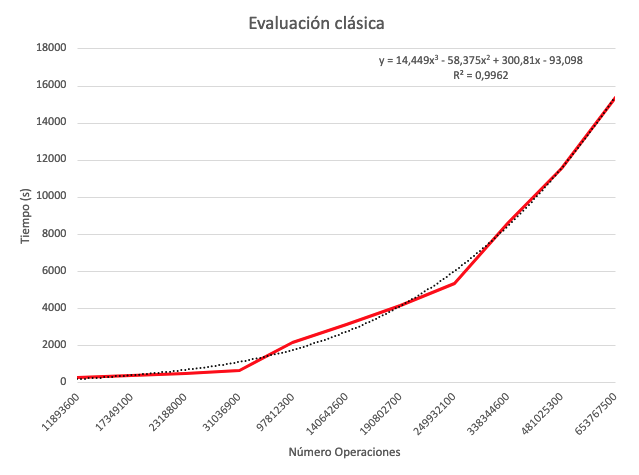
\includegraphics[scale=0.52]{graficos/eval_clasic.png}
  \caption{Gráfico de resultados Evaluación Clásica}
\end{figure}

\begin{table}[h]
  \caption{Tabla de resultados con la evaluación clásica}
  \centering
  \begin{tabular}{|l|l|l|l|}
    \hline
    Aristas  & Evaluación & Llamadas  & Tiempo (ms) \\ \hline
    2451 & Clásica    & 11893600  & 269,86      \\ \hline
    2962 & Clásica    & 17349100  & 381,1       \\ \hline
    3421 & Clásica    & 23188000  & 502,8       \\ \hline
    3961 & Clásica    & 31036900  & 685,73      \\ \hline
    9916 & Clásica    & 97812300  & 2187,36     \\ \hline
    11889 & Clásica    & 140642600 & 3125,26     \\ \hline
    13844 & Clásica    & 190802700 & 4181,23     \\ \hline
    15849 & Clásica    & 249932100 & 5344,96     \\ \hline
    22563 & Clásica    & 338344600 & 8573,06     \\ \hline
    26899 & Clásica    & 481025300 & 11572,93    \\ \hline
    31364 & Clásica    & 653767500 & 15408,46    \\ \hline
  \end{tabular}
\end{table}

\newpage

\begin{figure}[h]
  \centering
  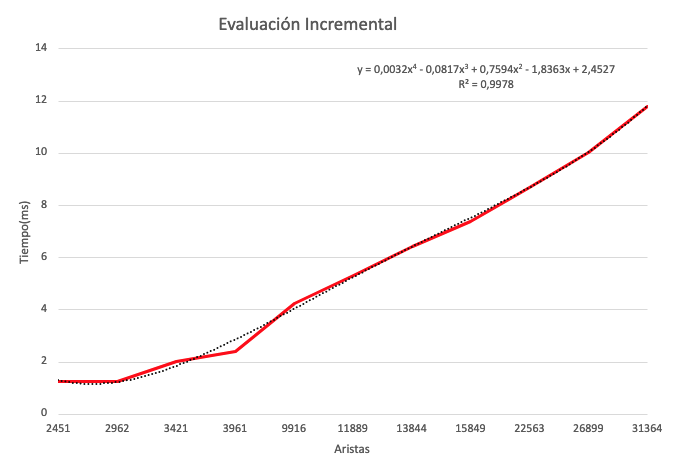
\includegraphics[scale=0.52]{graficos/eval_incr.png}
  \caption{Gráfico de resultados Evaluación Incremental}
\end{figure}

\begin{table}[h]
  \caption{Tabla de resultados con la evaluación incremental}
  \centering
  \begin{tabular}{|l|l|l|l|}
    \hline
    Aristas  & Evaluación  & Llamadas & Tiempo (ms) \\ \hline
    2451 & Incremental & 192,66   & 1,26        \\ \hline
    2962 & Incremental & 236,1    & 1,26        \\ \hline
    3421 & Incremental & 271,56   & 2,03        \\ \hline
    3961 & Incremental & 311,46   & 2,4         \\ \hline
    9916 & Incremental & 401,033  & 4,23        \\ \hline
    11889 & Incremental & 478,86   & 5,3         \\ \hline
    13844 & Incremental & 550,13   & 6,43        \\ \hline
    15849 & Incremental & 630,96   & 7,4         \\ \hline
    22563 & Incremental & 593,96   & 8,7         \\ \hline
    26899 & Incremental & 718,53   & 10,03       \\ \hline
    31364 & Incremental & 838,866  & 11,8        \\ \hline
  \end{tabular}
\end{table}



Considerando los resultados de las graficas déspues de experimentar la corrida con grafos bipartitos completos, el comportamiento es del orden polinomial. Esto es debido al aumento del problema en cada ejecución.\\

En la segunda grafica se observa la tendencia lineal de la evaluación incremental, no obstante no podemos considerar que una es mejor que la otra. Cabe señalar que no atacamos el problema \textbf{max bandwidth} de manera de busca el óptimo y sólo realizamos el intercambio de posiciones evitando recalcular toda la lista de pares de aristas adyacentes. Pero puede ser piedra angular para aplicarlo a una metaheurística de manera de ir encontrando una mejor solución respecto a los objetivos del \textbf{max bandwidth}


\newpage
\section{Aprendizajes}

Al tomar el curso de Análisis y Diseño de Algortimos, sabía del reto de cursar una clase fuera de mi línea, pero de mi interés. Sé de la importancia de conocer algoritmos y estructuras de datos como herramientas para la resolución de problemas, herramientas disponibles cuando se necesiten al momento de desarrollar un proyecto.\\

Gracias a tomar el curso, logré acercarme al estudio de grafos más allá de lo visto en matemáticas discretas. El poder manipularlo, explorarlo, logrando así obtener una herramienta poderosa como es la estructura y representación de un grafo. Es bien sabido que varios problemas en nuestra vida cotidiana se pueden llegar a representar con grafos. Tanto fué mi interés que traté de llevarlo a mis otras materias.\\

Con ayuda del curso obtuve ese empujón que siempre quise tener para comenzar a programar en C++. Salirme de mi zona de confort, y ampliar mis conocimientos en lenguajes que no pasan de moda y que son altamente portables.\\

Aunque es un hecho que no repartí mi tiempo de forma equitativa entre esta materia y las otras, logré llevar los conocimientos de clase a los demás proyectos. Cambiando así mi paradigma a utilizar algoritmos vistos en clase.\\

Sé que mi desempeño pudó ser mejor y a pesar de los altibajos y el apoyo del Dr. Eduardo Arturo Rodriguez Tello, a quién agradezco por sus palabras de aliento cuando imaginaba que mi proyecto de estudiar una Maestria en Ciencias se venía abajo. Siendo eso ya no es un problema para mí, ya que considero que los conocimientos adquiridos este cuatrimestre serán de gran ayuda para el desarrollo de códigos adaptables y modulares al momento que me toque regresar a la vida laboral.\\

No espero obtener una buena calificación, pero reconozco el esfuerzo que dedique en la matería, y sólo espero obtener una nota mínima aprobatoria a pesar de mis entregas tardías que pudieran confundirse con desinterés.

%------------------------------------------------
\section{Conclusiones}

Como se mencionó en clases, la algorítmica es reconocida como la pieda angular de las ciencias computacionales. El saber de ellas, y aplicarlas es de suma importancia para el desarrollo de códigos limpios.\\

El manejo de abstracciones de clases, las estructuras de datos para generar algoritmos eficientes es de suma importancia. Un ejemplo de ello fué en el presente trabajo donde se logró reducir considerablemente el tiempo de ejecución con simples estructuras aprovechando los ciclos donde se forma la información, para así hacer uso de ellos en pasos posteriores, aunque pueda afectar en el crecimiento espacial, es algo con el que podemos llegar a lidiar. Quitandonos así de tiempos de ejecuciones altos, logrando eficienciar nuestro código.

%----------------------------------------------------------------------------------------
%	REFERENCE LIST
%----------------------------------------------------------------------------------------
\newpage
\begin{thebibliography}{0} % Bibliography - this is intentionally simple in this template
\bibitem{calamoneri} New results on edge-bandwidth, Theoretical Computer Science, Tiziana Calamoneri(a), Annalisa Massini(a), Imrich Vrto(b), (a) Computer Science Department, University of Rome, (b) Institute of Mathematics, Slovak Academy of Sciences, Department of Informatics, Bratislava, 2003
\bibitem{balogh} On the edge-bandwidth of graph products, Theoretical Computer Science, József Balog(a), Dhruv Mubayi(b), András Pluhár(c), (a) Department of Mathematical Sciences, The Ohio State University, Columbus OH, USA, (b) Department of Mathematics, Statistics, and Computer Science, University of Illinois, Chicago IL, USA, (c) Department of Computer Science, University of Szeged, Hungary, 2006
\bibitem{SAP} Some Applications of Graph Bandwidth to Constraint Satisfaction Problems, Ramin Zabih, Computer Science Department Stanford University, Standford California \href{https://www.cs.cornell.edu/~rdz/Papers/Z-AAAI90.pdf}{ver artículo}
  
\end{thebibliography}

%----------------------------------------------------------------------------------------

\end{document}
